\section{PPO}\label{PPO}

We construct PPO using Tensorflow / Keras library.

The PPO model has 2 networks: actor and critic network. Actor network is the policy network and the loss function is the PPO loss, calculated as (pseudo-code):
\begin{lstlisting}
ratio = exp( log(newpolicy_pi)  - log(oldpolicy_pi) )

# following the formulas from the PPO paper
val_1 = ratio * advantages
val_2 = K.clip(ratio, min_value=1 - clipping_val, max_value=1 + clipping_val) * advantages

actor_loss = - mean(K.minimum(val_1, val_2))
\end{lstlisting}

Here we calculate advantages using the recursive formula for GAE (pseudo-code):
\begin{lstlisting}
delta = rewards[i] + gamma * values[i + 1] * masks[i] - values[i]
gae = delta + gamma * lmbda * masks[i] * gae
\end{lstlisting}

We train the PPO over 100 episodes, and let it play until ``done'' and for max. 100 steps inside each episode.

In each episode, after experienced is collected, the actor and critic nets are updated and environment reset.

Early-stopping is introduced when the system starts scoring positive reward (goal).

We show the value (critic) and policy (actor) loss plot as function of training episodes in figure \ref{fig_ppo_losses} (a) and (b), respectively.

After training is completed, we run the game for 100 episodes, each time allowing for a max. of 100 ``moves'' before terminating the game. We record rewards and plot in figure \ref{fig_ppo_rewards} (a). The cumulative rewards over 100 testing steps is shows in figure \ref{fig_ppo_rewards} (b). 

\begin{center}
\begin{tabular}{lclc}
(a) &
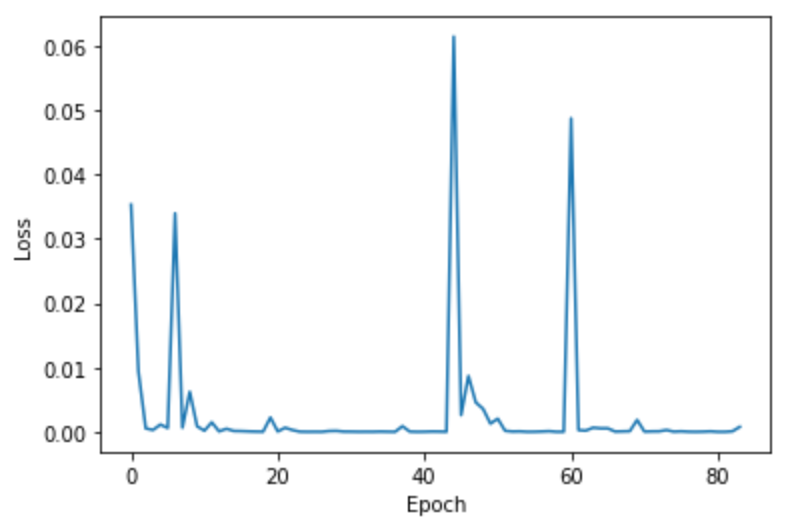
\includegraphics[width=5cm]{fig_ppo_loss_critic.jpg}
& (b)
&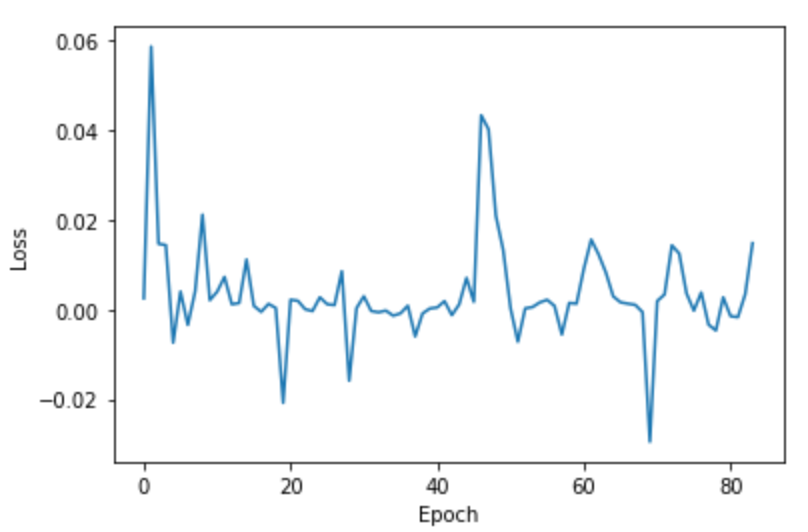
\includegraphics[width=5cm]{fig_ppo_loss_actor.jpg}
\end{tabular}
\captionof{figure}{(a) critic (value) and (b) actor (policy) PPO model training loss.}
\label{fig_ppo_losses}
\end{center}

\begin{center}
\begin{tabular}{lclc}
(a) &
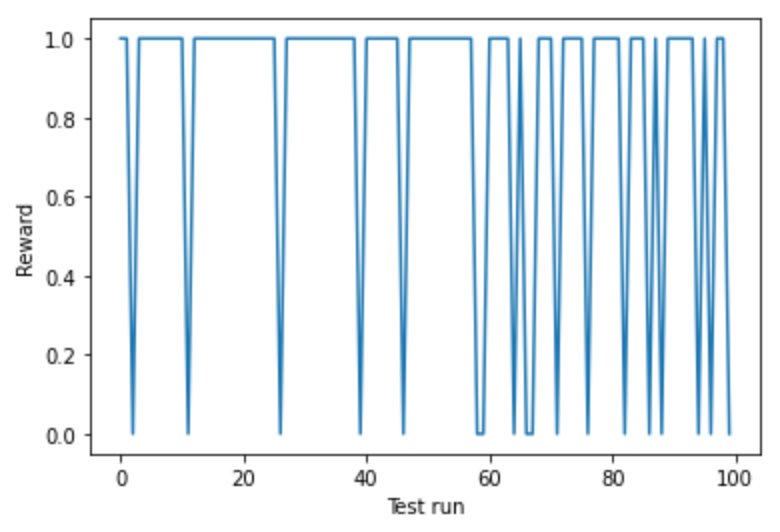
\includegraphics[width=5cm]{fig_ppo_reward.jpg}
& (b)
&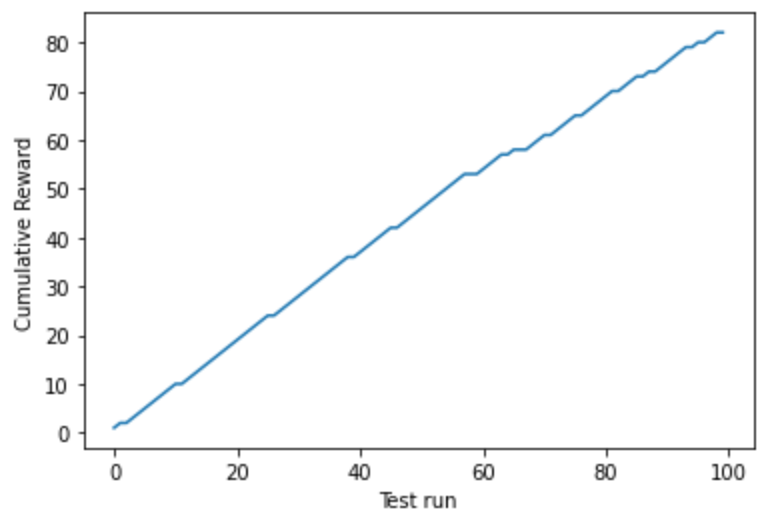
\includegraphics[width=5cm]{fig_ppo_reward_cum.jpg}
\end{tabular}
\captionof{figure}{Rewards for 100 test steps of the PPO model. (a) shows the rewards, while (b) is the cumulative reward.}
\label{fig_ppo_rewards}
\end{center}